\chapter{The Compact Muon Solenoid Experiment at the LHC}
\label{ch:detector}
\section{The Large Hadron Collider}

The Large Hadron Collider (LHC) is a double-ring circular synchrotron at CERN designed to collide two proton beams with a centre of mass energy $\sqrt{s}$  = 14 $\tev$ at a final design luminosity of $10^{34}$cm$^{-2}$s$^{-1}$. The energy and luminosity have been chosen with the aim of discovering new physics at the TeV scale, out of reach to previous experiments, where theories predict new physics both within and outside the Standard Model. It will also be used to collide heavy lead ions (Pb$^{82+}$) to an energy of 2.76 $\tev$  per nucleon, in specific runs, with the purpose of investigating QCD matter at energies 30 times higher than previous experiments. 
The LHC has unparalleled reach in the search for new physics, not only due to the significant increase of energy over the Tevatron, the previous record holder, but also due to the intensity of the beams delivered. The number of events produced by a given physical process depends proportionally on its cross section $\sigma$, and therefore proportional to $\sqrt{s}$ and the luminosity $\lumi$, which has the dependence shown in Equation \ref{eq:lumi} below~\cite{LHCDesign}:

\begin{equation}
n = \lumi \sigma, \hspace{.75in} \lumi = \frac{N_{b}^{2} n_{b} f_{rev} \gamma_{r}}{4 \pi \epsilon_{n} \beta^{*}}F
\label{eq:lumi}
\end{equation}

where $N_{b}$ is the number of particles in a single bunch, $n_{b}$ is the number of bunches in a beam, $f_{rev}$ the frequency of revolutions, $\gamma_{r}$ is the relativistic gamma, $\epsilon_{n}$ is the beam emittance and $\beta^{*}$ is the beta function associated with the collision point. The geometric luminosity function F provides a reduction factor based on the beam crossing angle, and depends on the full crossing angle at the IP $\theta_{c}$, and the transverse and longitudinal RMS beam dimensions $\sigma_{*}$ and $\sigma_{z}$ with the following dependency:
\begin{equation}
F^{2} = \frac{1}{1+(\frac{\theta_{c} \sigma_{z}}{2\sigma_{*}})}
\label{eq:lumi2}
\end{equation}

Situated in the tunnel of the previous $e^{+}e^{-}$ machine LEP located underneath the Franco-Swiss border,  the LHC is mostly circular with a circumference of 27km, consisting of 8 arced sectors connected by 8 straight sections in which are the numbered Interaction Points (IP), where the two beams circulating in opposite directions can be made to collide. To bend the protons around the rings, the two beams experience opposite dipole fields from one another, and have two separate vacuum systems. As the tunnel has restricted space available, the dipole magnets are twin bore with two coils and, but share the same structure and cryogenics. The 1232 superconducting dipole magnets present must produce a field in excess of 8T due to the high momentum of the protons, and thus have a high current and must be cooled below 2K by liquid helium to ensure safe operation. The beams are non-continuous, grouped in ``bunches" at intervals. In the straight sections the two beams share the same beam line and can be directed to coincide at the IP's. In order to maximise the number of interactions, quadropole magnets are used to focus the beam providing a minimum cross section at the point of interaction.

At four of these IP's are located the four main detectors that analyse the data from collisions: the two high luminosity experiments ATLAS (A Toroidal LHC Apparatus) at IP1 and CMS(Compact Muon Solenoid) at IP5 are multi-purpose detectors analysing the p-p collisions for signs of new physics. At IP8 the LHCb (LHC beauty) detector looks for CP violation and other rare decays in a forward detector with lower luminosity runs, and ALICE (A Large Ion Collider Experiment) at IP2 will investigate the lead-lead ion collisions. The locations of the detectors in the LHC ring is shown in Figure \ref{fig:LHC}~\cite{LHCConcept} .

\begin{figure}[htbp]
\centering
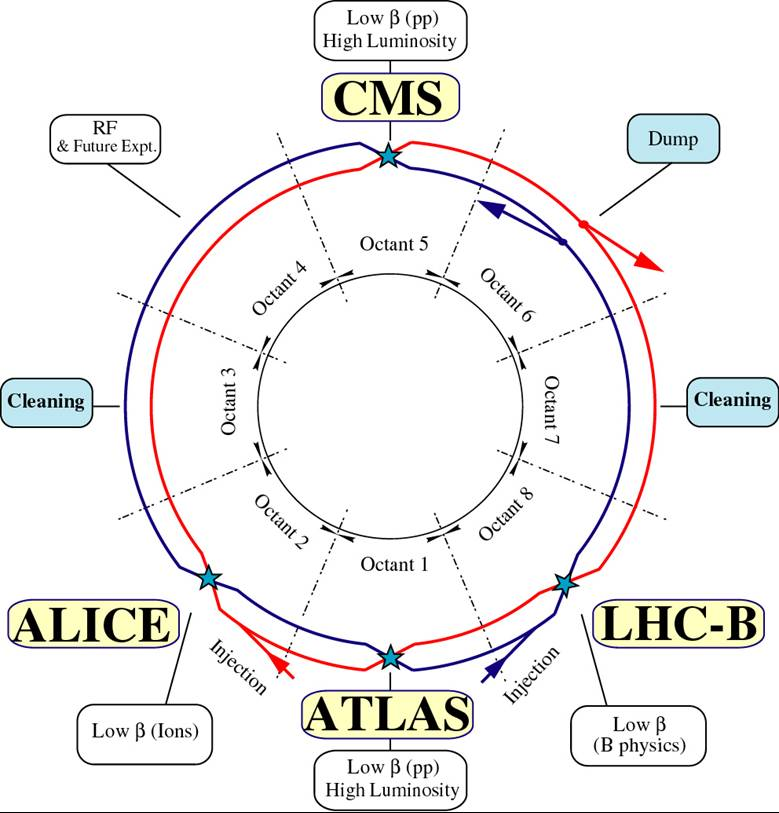
\includegraphics[width=0.85\textwidth]{Figures/Detector/lhc-schematic}
\caption{Schematic of the LHC ring and the location of the major experiments.}
\label{fig:LHC}
\end{figure}


The magnets are optimised for beams of a certain energy range, and therefore the protons cannot be fully accelerated in the LHC. Therefore the supply of protons are delivered through a series of other machines that make up part of the CERN accelerator complex, the layout of which is shown in Figure \ref{fig:LHCinject}. 

A beam of 50MeV protons is created in LINAC2, in 6 bunches, and each bunch is then split into 12, resulting in 72 bunches which are fed into the Proton Synchrotron Booster. After accelerating to an energy of 1.4~GeV they enter the Proton Synchrotron, where they are accelerated to 26~GeV. Then 2-4 sets of 72 bunches are fed into the Super Proton Synchrotron. Now 144-288 bunches, they are accelerated to 460~GeV ready of injection into the LHC. Twelve of these sets are injected into the LHC, directly into both rings, giving a nominal bunch density of 2808, with a spacing of 25\,ns. This process takes around 20 minutes, and then the LHC takes a further 20 minutes to ramp the protons up to the desired energy by raising the current of the dipoles. The magnets preventing the beams coinciding in the detectors are turned off and stable collisions occur. The luminosity falls regularly as the run progresses as protons are lost in collisions, and after 6-12 hours, it has fallen below an acceptable level, and the beam is dumped before repeating the process again. 

Using these short runs of high luminosity it is possible for the LHC to take large amounts of data, and assuming 200 days of data taking a year  at design luminosity the machine will be able to deliver 100~fb$^{-1}$ a year. As part of the early phase of operation the machine was operated in 2010-2011 at 3.5~TeV per beam, $\sqrt{s} = $7~TeV, in order to protect the magnets, and is not expected to run at full energy until 2014. The 2011 run delivered 5.727~fb$^{-1}$ data, the first 1.1~fb$^{-1}$ of which was delivered by the end of June, and is considered for this thesis.

\begin{figure}[htbp]
\centering
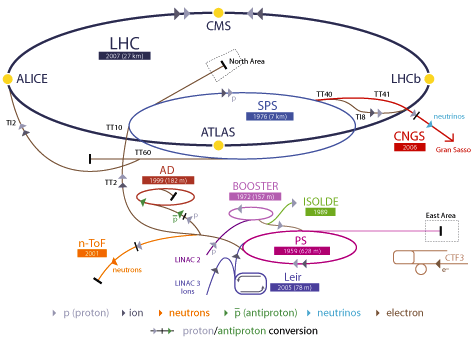
\includegraphics[width=0.8\textwidth]{Figures/Detector/injection}
\caption{Layout of the CERN accelerator complex, illustrating the relationship between the LHC and its supporting accelerators tasked with delivering proton beams at 460~GeV.}
\label{fig:LHCinject}
\end{figure}



\section{The Compact Muon Solenoid}

The Compact Muon Solenoid (CMS) is one of the two high-luminosity multi-purpose detectors at the LHC, designed to capitalise on the full range of physics opportunities available as a new energy scale is probed. These goals are pursued through the design and construction of the detector and development of software for the reconstruction of physics objects. The detector is constructed of several detector sub-systems contained inside and wrapped in layers around a central 13m long 4T super conducting solenoid as shown in Figure \ref{fig:CMS_Struct}. 

The detector is 21m long, 15m wide, weighs 14000 tonnes and consists of five wheel-like barrel sections and two end-caps. In order for CMS to search for new physics among the high Standard Model backgrounds, it is of key importance to develop a detector which has excellent energy and momentum resolution and particle identification. Different particles interact differently with matter and therefore a number of sub-detectors are needed in order to gather all the relative information. These data are then combined in order to reconstruct the objects. 

\begin{figure}[htbp]
\centering
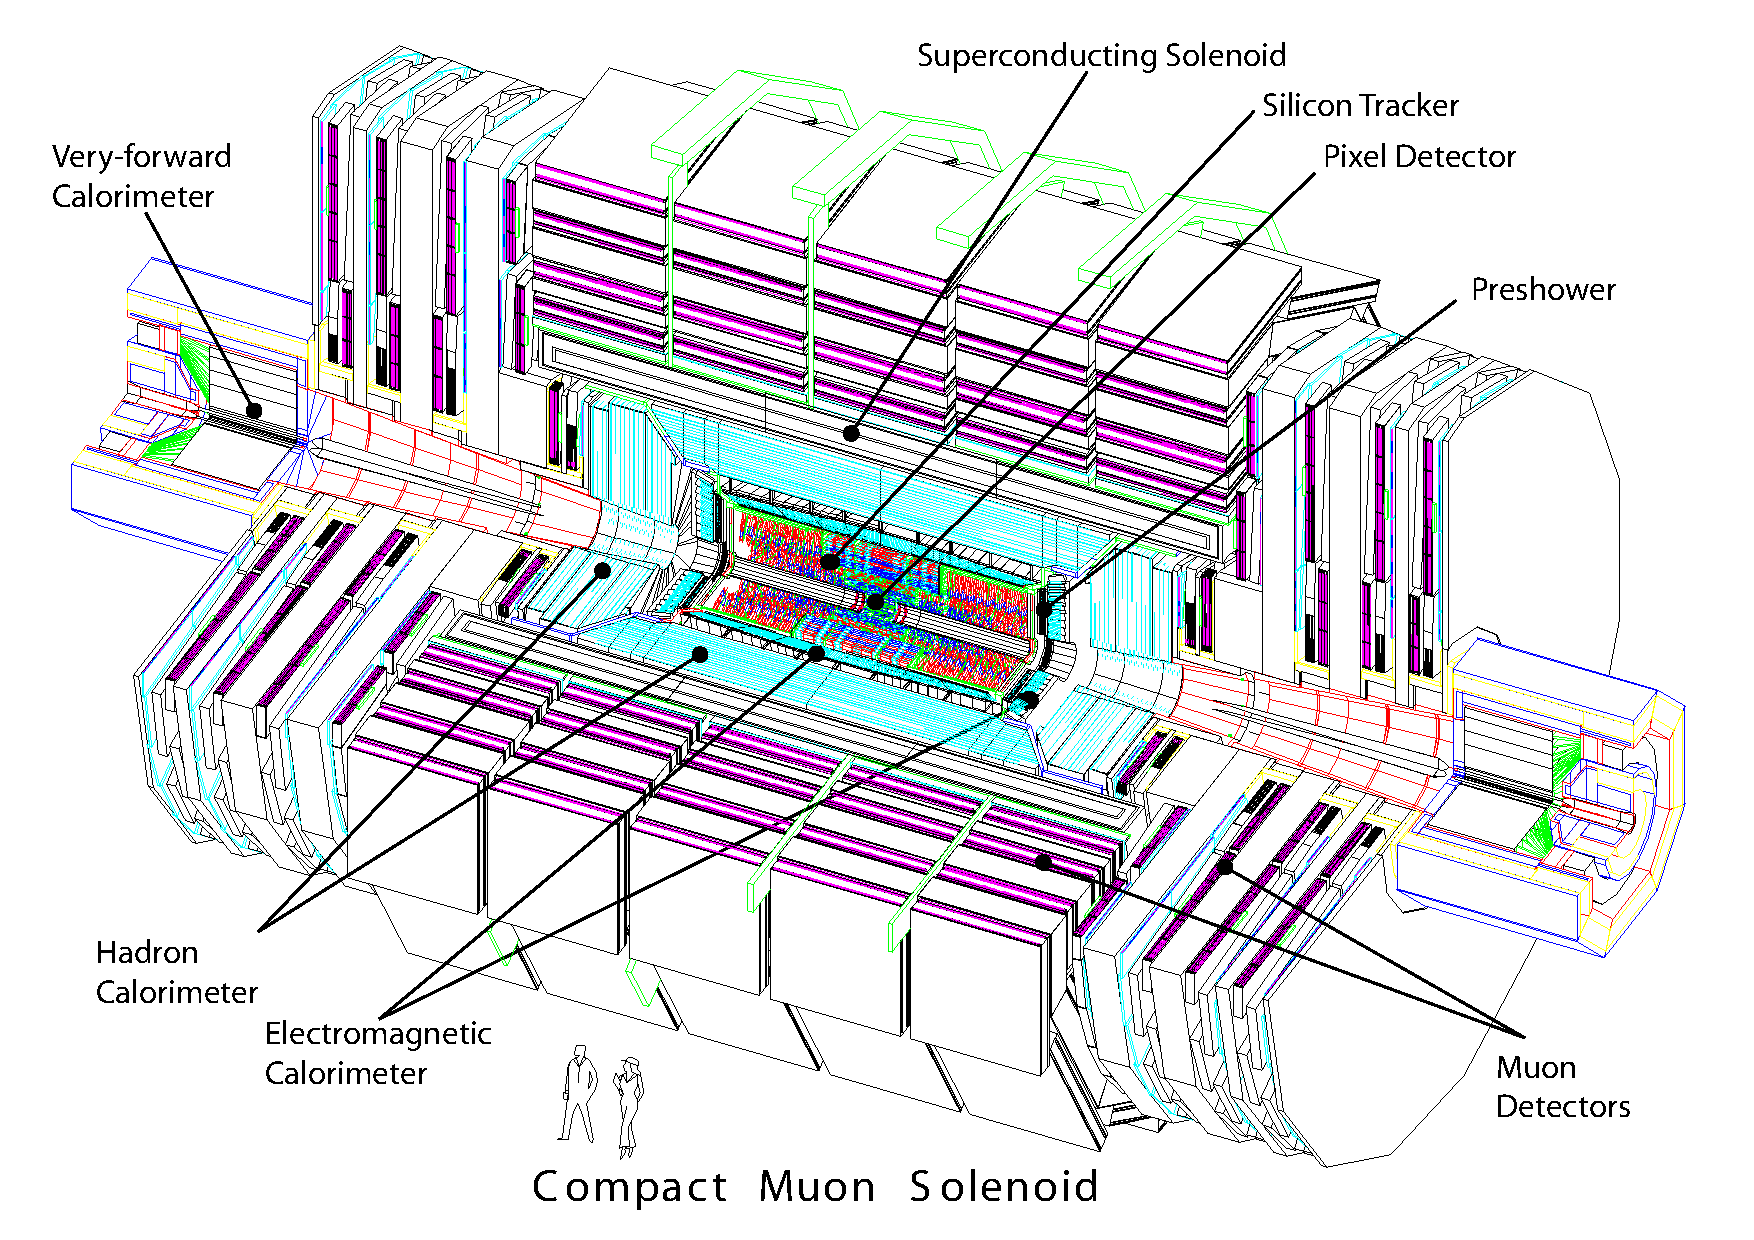
\includegraphics[width=0.9\textwidth]{Figures/Detector/CMS_Structure}
\caption{A cutaway diagram of the CMS detector structure identifying the main individual sub-systems.}
\label{fig:CMS_Struct}
\end{figure}

The high magnetic field was chosen in order to achieve the bending power necessary for good charged particle momentum resolution. The inner bore of the solenoid is large enough that the inner tracker and the calorimeters are located inside, which minimises the material the particles pass through before entering the calorimeters. This improves the energy measurement resolution. Four muon ``stations" of aluminium drift tubes are integrated within the iron magnetic field return yoke. The full design description can be found in the CMS Technical Design Proposal \cite{CMSTDP}. As different particles pass through the detector they interact in the sub-systems depending on their type. A transverse slice through the detector illustrating the path through the machine of each type of particle is shown in Figure \ref{fig:CMS_Slice} 





\begin{sidewaysfigure}
\centering
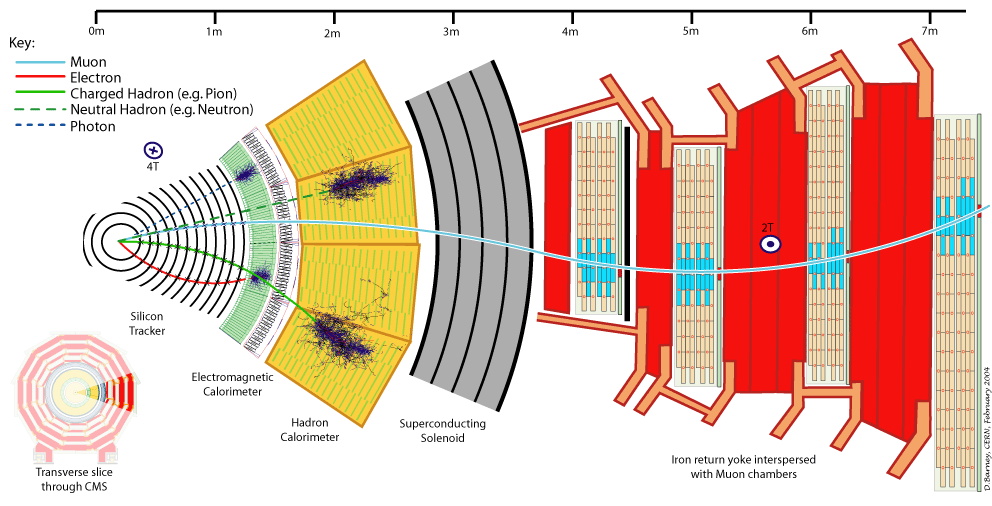
\includegraphics[width=1.\textwidth]{Figures/Detector/CMS_Slice}
\caption{Transverse slice through the CMS Detector showing the path of each type of particle and how it interacts with the sub-detectors.}
\label{fig:CMS_Slice}
\end{sidewaysfigure}
\subsection{Coordinate System}

The coordinate system chosen by CMS uses the nominal interaction point within the detector as the origin. The x-axis points radially inwards to the centre of the collider ring, and the y-axis points vertically upward. The z-axis then points in the direction of the anti-clockwise beam. The azimuthal angle $\phi$ is defined as the angle from the x-axis in the x-y plane, and the polar angle $\theta$ from the z-axis. However, it is common convention to express $\theta$ in terms of the Lorentz Invariant quantity, pseudorapidity~\begin{math}
\eta = -\ln \tan (\theta / 2) 
\end{math}, as particle production is approximately uniform in $\eta$. The transverse components of the energy and momentum, denoted $E_{T}$ and $p_{T}$ are then calculated from the $x$ and $y$ components. 



\subsection{Superconducting Magnet}

The geometry of the magnetic field is integral to the design and cylindrical structure of the CMS detector, as it uses a global solenoidal magnet. A strong magnetic field is essential to the design of a detector, bending charged particles in order to measure their charge and momentum. In order to ensure that the curvature is significant even with particles of high momentum, the CMS solenoid is designed to be capable of delivering a homogenous field of 4\,T within its volume. Consisting of four layers of NbTi coils, in a vacuum with a cryogenic system maintaining a temperature of 4.5\,K, the solenoid has a diameter of 5.9\,m and length 12.5\,m, and when operating at full current is cable of storing 2.6~GJ of potential energy.

As the solenoid is so large, not only the inner tracking system but also both calorimeter sub-detectors can be accommodated in the interior, giving significant advantage to electromagnetic and jet energy resolution as particles will not have traversed the high-density magnet coil before these measurements are taken. The flux is returned with a large iron yoke of $10^{7}$~kg, surrounding the inner magnet and built with a barrel of 5 wheels, and two end-caps each containing three disks. The muon system is built within the iron return yoke, in order to take advantage of the reverse magnetic field produced in the outer region, and thus follows the same structure. The drawback of a solenoidal field is that it has strong inhomogenity in the end-caps, affecting the performance of the muon subsystem, which shall be discussed later.


\subsection{Tracker}



The first sub-detector encountered by particles is the multi-layer silicon tracker, which records precise information about the path of charged particles bending under the magnetic field. The inner layers are placed as close to the interaction point as possible in order to distinguish the primary interaction from secondary vertices of particles with significant lifetimes. This is particularly important in the case of identifying B mesons, which can travel a measurable distance before decaying.  

The tracker is divided into regions defined by the radius r from the interaction point, as the expected particle flux decreases rapidly as the radius increases. This is due not just to the increase in area of the solid angle, but also to the high magnetic field, which causes low momentum particles to have small radial helical trajectories.

Nearest to the primary vertex at 4\,cm where the expected particle flux is at its highest ($\sim10^{8}$\,cm$^{-2}$\,s$^{-1}$) is the pixel detector which consists of 66 million silicon pixels of size 100 $\times$150\,\textmu m$^{2}$ arrayed in three barrel layers and two end-cap disks. This region is laid out to optimise the resolution in determining the vertex position, delivering a hit resolution of $\sim$10\,\textmu m in the r-$\theta$ plane and $\sim$ 20\,\textmu m in the r - z plane. Pixel detectors have the advantage of being able to measure all three coordinates of the particle simultaneously. However this requires a large number of readout channels and drives the costs of construction up. For this reason pixel detectors are chosen for the innermost region where the flux is highest, while the rest of the detector is composed of silicon micro-strip devices. 

Outside of the pixel detector lies the silicon strip tracker with its first layer located at r = 20\,cm. It is divided into two parts, the inner and outer components. As the flux of particles expected is lower than in the pixel detector, the use of 11.4 million silicon strips allows the desired granularity while minimising costs. Whilst these do now allow a simultaneous 3-coordinate measurement, some of the layers are constructed at known angles to the others and therefore combined together all three coordinates can be measured. The inner region, immediately outside the Pixel tracker, is composed of four barrel layers (TIB) and closed with three disks (TID) on each end, occupying the region up to r~=~55\,cm, where the microstrip sensors are 320\,\textmu m thick oriented along the beam line in TIB and radially in the TID. The outer region has 6 barrel layers (TOB) further apart than in the inner sector, and closed with 9 end-caps (TEC) on the end of the barrel, extending out to r~=\,116cm. The strips here are 500\,\textmu m thick.

In total the tracker covers a total area of 205m$^{2}$ with 76 million channels and provides a transverse momentum measurement for high momentum tracks with resolution 1 - 2\,\% in the region $|\eta| <$ 1.6.



\subsection{ECAL}

Immediately outside of the tracker, and still within the magnet core, sits the Electromagnetic Calorimeter (ECAL), used to measure the energy of electrons, photons and pions via the energy they lose through radiation. Electrons lose their energy in the material through \textit{bremsstrahlung}, and photons by decaying to an electron-positron pair. Using a hermetic homogenous calorimeter of scintillating crystals, this energy can be converted to scintillation light which is picked up by a light sensitive detector. 

The use of high density crystals allows a fast calorimeter which has fine granularity and is radiation resistant, requirements which are essential in the LHC environment. After rigorous research and development, lead tungstate ($PbWO_{4}$) crystals were chosen as the optimal solution to the requirements of LHC operation, due to a number of desirable characteristics. The extremely short radiation length $X_{0}$ = 0.89\,cm allows the construction of a compact ECAL which therefore can reside within the solenoid, hence reducing the amount of material particles have to pass through before reaching the calorimeter. In addition, the material has a small Moliere radius (2.2cm) meaning the transverse size of the electromagnetic shower is narrow, leading to good shower position resolution and separation. It is also essential that a fast scintillator is used, in order to distinguish between bunch crossings. In crystals of PbWO$_{4}$ 80\% of the scintillation light is emitted within 25ns, the bunch spacing of the LHC. Finally the crystals are hard to radiation, as their method of scintillation is resistant to radiation damage. 

The ECAL is structurally divided into three distinct regions, the End-caps (EE), the Barrel (EB) and the Preshower (PS), which together cover a pseudorapidity range $|\eta| \leq$3. The ECAL Barrel is a cylindrical arrangement of 61200 PbWO$_{4}$ crystals covering the pseudo rapidity range $|\eta| \leq$ 1.479 with a granularity of $\Delta \eta \times \Delta \phi = 0.0174 \times 0.0174$. The radius to the front-face of the crystals is 1.29 m. 


The ECAL is closed by two identical end-cap regions, which cover the range 1.479 $\leq |\eta| \leq$ 3 at the margins of the barrel, each consisting of 7324 crystals divided into two halves, or \textit{Dees}. Precision energy measurements are possible up to $|\eta|$ = 2.6, but crystals are include up to $|\eta|$ = 3 to assist the forward-direction energy-flow measurement. The end cap crystals are also wedge shaped with a square front face $28.62 \times 28.62$\,mm$^{2}$ and a square back face $30 \times 30$\,mm$^{2}$. The crystals point slightly away from the interaction point in order to make the end-caps hermetic, and are grouped mechanically into 5 $\times$ 5 super-crystals (SC). 

 The size of the crystals is chosen to reflect the properties and requirements, such that the front face surface area is 22 $\times$ 22\,mm$^{2}$ (the Moliere radius squared) and the longitudinal depth of the crystals is 230\,mm, which is 25.8 X$_{0}$ in the barrel, hence allowing a fine granularity and a compact ECAL. In the end-caps the presence of the PS allows for shorter crystals, of 220\,mm, corresponding to 24.7 X$_{0}$.

A additional component, the Pre-Shower is present in front of the end-caps covering a range of $1.653\leq |\eta|\leq2.6$ and consists of two layers of absorbing lead converters and silicon detectors. The primary function of the PS is to identify neutral pions that decay into two photons in the end-caps, which can fake high-energy photons. It also possesses a high granularity, and therefore is used to improve position determination of particles, and helps the identification of electrons against minimum ionising particles. The two layers of the PS have their strips orthogonal to one another such that the first layer has vertical strips to measure the critical position, and the second horizontal strips for the horizontal position. 

The crystals are read out using photodetectors, which convert the scintillating light of the crystals into an electric signal. The crystals were chosen by a rigorous optimisation of the properties required, which results in a high-performance ECAL, however this material has a relatively low light yield. In order to overcome this, photodetectors designed for use in a magnetic field with intrinsic gain are used. Vacuum Phototriodes  (VPTs) are used in the end-caps. These are unsuitable in the central region due to high magnetic, but due to lower radiation levels Avalanche Photodiodes (APDs) are used. Both the crystals and the photodetectors are sensitive to temperature changes, so a stable temperature must be maintained. Radiation damage to the crystals decreases with temperature, but so do the thermal effects which result in recovery. The operational temperature, 18C is chosen as it is the point of equilibrium between damage and recovery.


The resolution of an ECAL can be described as a function of the energy E in GeV, shown in Equation \ref{eq:E-Res}, for energies below about 500 GeV~\cite{PDG}. Above this shower leakage from the back of the crystals become non-negligible. 
\begin{equation}
\left(\frac{\sigma}{E}\right)^2 = \left(\frac{S}{\sqrt{E}}\right)^2 + \left(\frac{N}{E}\right)^2 + C^2
\label{eq:E-Res}
\end{equation}
The stochastic term S represents fluctuations related to statistics, including photoelectron statistics and intrinsic shower variations. The noise term N takes into account electronic noise summed over readout channels, and the constant term C accounts for the uncertainty in calibration and the detector non-uniformity. Measurements from test beam reconstructed energy distributions show values for the terms to be S\,=\,2.8\,$\pm$\,0.1\,\%, N=0.12\,GeV and C\,=\,0.30\,$\pm$\,0.01\,\%. 


\subsection{HCAL}

Outside the ECAL lies the Hadronic Calorimeter (HCAL),  responsible for the measurement of the hadronic activity of an event. This also leads to a measurement of apparent missing energy from neutrinos or exotic particles, an important quantity in many searches for new physics. In order to measure the energy of hadrons in a compact space, a sampling calorimeter of interleaved layers of absorbers and scintillators is used. The absorbing material forces hadronic showering through nuclear interaction with heavy nuclei, and the active scintillating material then samples the showers of charged particles produced. The absorber material is described by the interaction length $\lambda_{I}$, the distance a hadron will travel through the material before it has lost roughly 63\% of its energy through nuclear interactions.

 The HCAL is divided into several sections, defined by pseudo-rapidity in order to optimise the resolution under different conditions. Within the space between the ECAL and the magnet coil lie the HCAL Barrel (HB) at $|\eta| < 1.305$, and the HCAL End-Caps (HE) at $1.305 < |\eta| < 3.0$, hermetically joined to completely surround the ECAL. In order to increase the hermicity of the HCAL, and therefore improve the accuracy of the missing energy measurement, the two elements of the HCAL Forward calorimeter (HF) overlap with the HE and extend the range in pseudorapidity to $|\eta|<5$. There is also a complimentary layer of scintillators on the outside of the coil, known at the HCAL Outer (HO).  This provides shower containment in the central region, where the number of interaction lengths travelled by a particle is at its lowest~\cite{HCALTDR}.


\begin{figure}
\centering
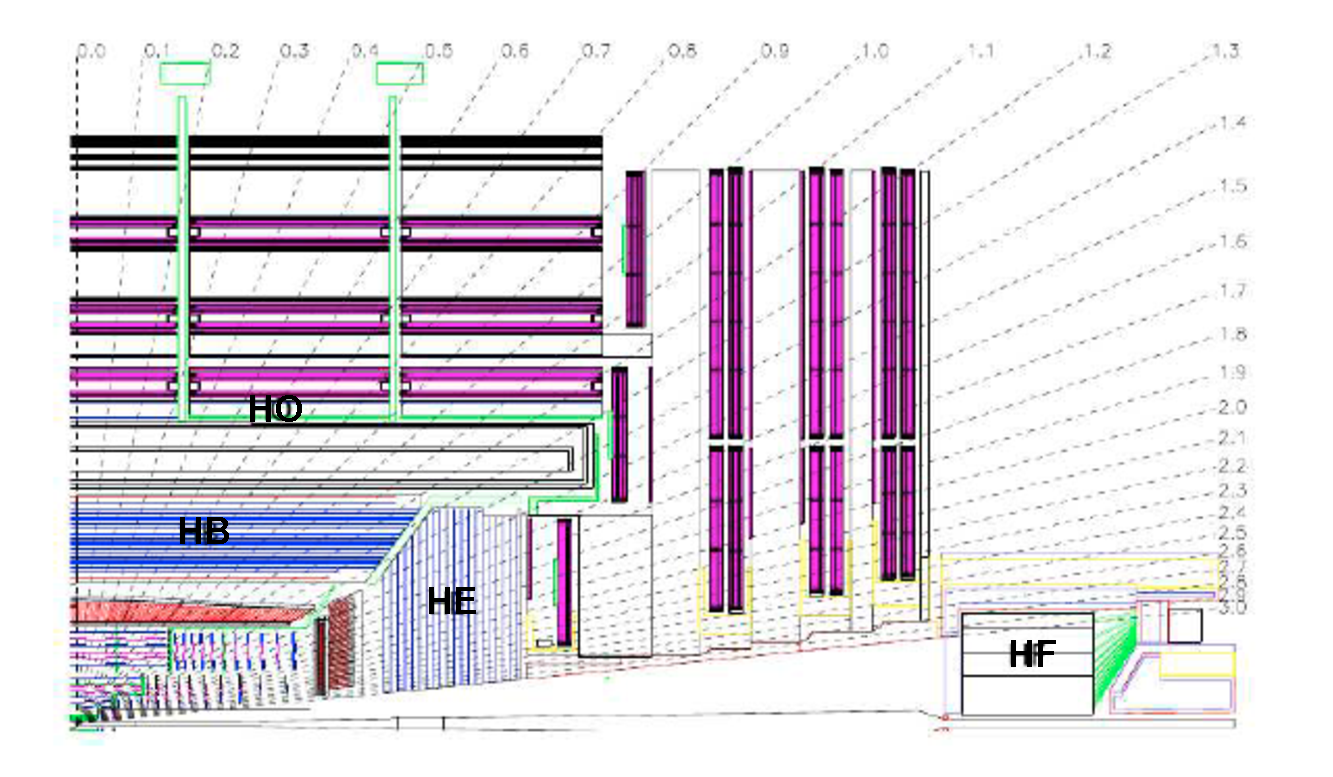
\includegraphics[width=0.8\textwidth]{Figures/Detector/HCAL}
\caption{Diagram of one quadrant in the r-$\theta$ plane showing the locations of the components of the HCAL: HB, HE, HO and HF, with lines of constant $\eta$ shown.}
\label{fig:HCAL}
\end{figure}


The barrel consists of two halves each with 18 identical azimuthal wedges, extending outwards 0.96m. Each wedge has 17 layers of 3.7mm thick plastic scintillator, interspersed with brass absorber plates, with the exception of the innermost and outermost absorbers, made from stainless steel to add structural stability. Directly behind the ECAL is placed the first active layer, with more than double the scintillator thickness (9mm) to actively sample the particles traversing the support material between the ECAL and HCAL. The final layer also has this thickness to catch showers that form late in the absorber. 

A similar structure makes up the end-caps with 18 wedges in $\phi$ containing 19 active plastic scintillators with brass absorbers between. The number of interaction lengths travelled by particles in the HB and HE is dependent on the $\eta$ of the particle, and while it is 10 at high $\eta$, in the central region this is as low as 5. In order to compensate for this, an outer barrel detector is added in the range $|\eta| <$ 1.26 consisting of two layers of scintillating material outside the magnet, and therefore utilising the coil as an absorber. This extends the total thickness of the full calorimeter to at least 11.8 interaction lengths. 

The design of the forward calorimeters is driven by the need for radiation hardness, as the region closest to the beam line has an energy density up to seven times greater than in the central region. Thus absorbers made of stainless steel and active scintillators of quartz fibres are chosen. Twelve $\phi$ wedges are located 11.2m from the point of interaction, with the fibres parallel to the beam.

Measurements of hadron energies in the region $| \eta| < 3.0$ rely not only on the HCAL setup described, as a significant fraction of hadrons with have begun to shower while travelling through the ECAL, which contributes around one interaction length.  The hadronic component of these showers will continue on into the HCAL, but much of the initial electromagnetic activity can be contained in the ECAL, thus use of measurements in both calorimeters are combined to reconstruct the true energy of a hadron. Using test beams over a range from 2 to 350 GeV the resolution for the reconstruction of hadron energy for the HCAL and ECAL combined is given by the following equation~\cite{HCALTestBeam}.
\begin{equation} 
\left(\frac{\sigma}{E}\right)^2 = \left(\frac{84.7\%}{\sqrt{E}}\right)^2 + \left(7.4\% \right)^2 
\label{eq:H-Res}
\end{equation}


\subsection{Muon System}

Interleaved in the iron return yoke of the detector are the components of the Muon System (MS), an important design feature giving CMS its middle initial. Many new physics signatures at high energy have final states with high momentum muons, and therefore accurately measuring these is crucial for many analyses, including Higgs and SUSY channels. As muons are high mass leptons they interact little in the calorimeters, and thus retain a high percentage of their energy by the time they reach the iron return yoke. Putting the MS here far away from the interaction point allows finer precision, utilising the high magnetic field to bend even high momentum muons, and measuring the bending angle.

Muon momentum resolution using the MS is dominated at low energies (0 $< p^{\mu}_{T} < $ 200 GeV) by the multiple scattering that occurs in the material prior to the first muon station, and therefore a better resolution could be obtained using the tracking system. However, it is possible to use the muon trajectory after the yoke to extrapolate back to the interaction point. Using the tracker and muon system together improves identification and measurements, especially as any particle detected in the MS is expected to be a muon, as other particles are stopped earlier in the detector~\cite{MuonTDR}. 

Built within the iron yoke the MS shares the same structural layout, constructed in five barrel wheels, and two end-caps, together covering the region $|\eta| < 2.4$. As a large area must be covered, a silicon based setup such as the inner tracker would be too expensive, hence gaseous detectors are chosen. In the barrel region ($|\eta| < 1.2$) Drift Tubes (DT) are used, and in the end-caps ($0.9 < |\eta| < 2.4$) Cathode Strip Chambers (CSC) are preferred, both of which offer good position resolution, although they have a long response time. In order to provide redundancy in the trigger system an additional third element is added in both regions, the Resistive Plate Chambers (RPC). These have a worse position resolution but benefit from a much shorter response time suited to identifying the bunch crossing. Combining the information from these complimentary RPCs with the DTs and CSCs gives rise to an efficient and robust trigger. The arrangement of the muon system is shown in Figure~\ref{fig:MuonSystem}, with the locations of each type of detector shown.

\begin{figure}
\centering
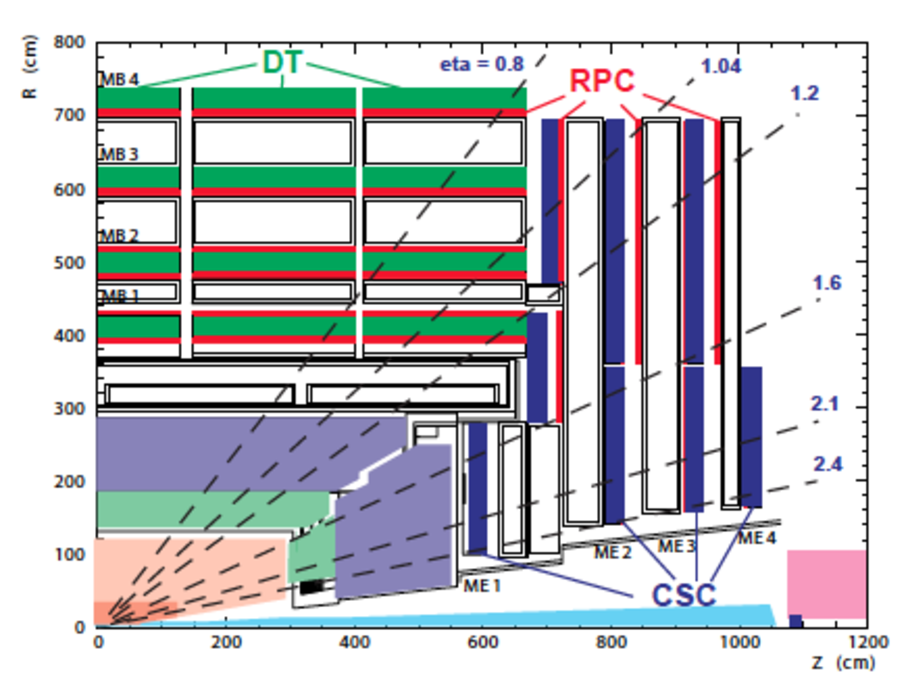
\includegraphics[width=0.6\textwidth]{Figures/Detector/MS}
\caption{The Muon system shown in the $r-\theta$}
\label{fig:MuonSystem}
\end{figure}

In the barrel, the magnetic field is uniform, and therefore allows the use of Drift Tube chambers.  Each of the five wheels are made up of 12 sectors, containing four chambers apiece, making up a full barrel of 240 chambers. The inner three chambers consist of three Super Layers (SL) using the first and third for the $\phi$ coordinate measurement and the second for the z coordinate. In the outer chamber,  there are only two SL's and these contribute only to the $\phi$ measurement. Four layers of drift tubes make up a SL, and each layer is shifted by half a cell from the one beneath, to ensure any particle trajectory meets some active material. Each tube contains an anode wire and cathode strips, and is filled with a gas mixture of 85\% Ar and 15\% $CO_{2}$ gas. The Ar atoms are ionised by a charged particle, and the resulting electrons and ions drift towards the anode and cathodes. Electrons reaching the wire are extremely excited by the high density field, which allows them to ionise further molecules, known as the ``avalanche effect". Thus an electrical signal large enough to be measured is produced. The drift distance is 21\,mm and the drift time is limited to $\sim$\,380\,ns by the gas chosen, corresponding to 16 bunch crossings.

Due to the aforementioned solenoidal magnetic field, the end-caps experience an irregular magnetic field, and a higher expected particle flux, and therefore drift tubes are not suitable. In this region 468 Cathode Strip Chambers are used, set out perpendicularly in four stations in each end-cap. Trapezoidal chambers consist of seven radially oriented cathode strips, and in between six planes of azimuthal anode wires. The gas filling the gaps is made up of 40\% Ar, 50\% CO$_{2}$ and 10\% CF$_{4}$, and the chambers work much in the same way as the DT's, with a high voltage applied to achieve the avalanche effect. As the wires and strips are almost perpendicular its possible to make a simultaneous measurement in r and $\phi$ by identifying the charge fraction in several cathode strips. 

In addition, the complimentary system of RPC's is installed in both the barrel and end-cap regions, providing extra information in the region $|\eta| < 1.6$. In the barrel there are 480 rectangular RPC's, with two layers per station, the inner two stations have one inside and one outside the DT's, and the outer two stations having both inside. The end-caps have overlapping trapezoidal chambers in the outer two concentric rings. These parallel-plate gaseous detectors have two thin gaps between plates, which are attached to high voltage to drive avalanche mode. The avalanche reaches the plates quickly, as the gas gaps have a small width, and so the measurement is made within $\sim$\,3\,ns, much smaller than the bunch crossing. The position resolution is adequate at the same time, and so the RPC's are used to contribute to the trigger, and also to map identified muons to a particular bunch crossing.

\subsection{Trigger}
\label{sec:detrig}
When running at design luminosity, the LHC will collide protons with a bunch crossing of 25ns, each of which will result in $\sim$\,20 interactions corresponding to a rate of 40MHz of data, or 40\,TB/s~\cite{TRIGTDR}. Not only is it impracticable for this volume of data to be stored, but much of this corresponds to unwanted events, where no new particles have been produced, as the cross-sections for interesting physics processes are several orders of magnitude lower than the inelastic p-p cross section. Hence these events must be whittled down into those which it is worthwhile to store. This is done by the trigger system that is divided into two components, the online hardware-based Level 1 Trigger (L1) which reduces the rate to that which can be routed from the buffer to the computing farm, and then the offline software-based High Level Trigger (HLT). 

The L1 trigger is driven by the amount of time that data at the incoming rate that can be stored in the buffer, before needing to be overwritten. At design luminosity this is 128 bunch crossings, $\sim$\,3\,\textmu s. Within this time the rate must be lowered to 100kHz, the acceptable rate for writing to the computing farm used for the HLT. This is accomplished using a tree system of triggers. First, the Regional Calorimeter Trigger (RCT) and Regional Muon Trigger (RMT) perform local reconstruction of objects (muons, electrons, photons, jets). The Global Calorimeter Trigger (GCT) and the Global Muon Trigger (GMT) receive these objects, and sort them using a number of criteria e.g. Energy, momentum, quality of identification. The top four of each type are sent to the Global Trigger, which uses this information along with global event measurements such as total momentum to decide if the event passes the L1 Trigger requirement. If so it is sent to the HLT, if not it is not stored and passes out of the buffer. 

The HLT essentially does the same thing as the L1 trigger, but is not driven by strict time requirements. Running on a large computer farm of multi-core computers, it has access to the entire readout data, and performs sophisticated calculations akin to those performed in physics analyses. Using partial reconstruction algorithms to clearly identify what objects are in an event, it is possible to filter according to a set of desired physics criteria.  The desired rate to store to tape is around 300Hz, and the HLT is designed and monitored constantly during data-taking to ensure the correct rate is achieved. In a given run a ``menu" of different trigger paths is included, to select different types of event and with different thresholds. Some require the presence of a certain object, such as a Muon. Others combine requirements, and these are called Cross-Triggers. For example a family of triggers exist that require a certain HT and MHT. Within this family there are several different thresholds, which go down as low as can be included in the menu without raising the rate prohibitively much. Thresholds that have a rate which is too high become ``pre scaled".
\subsubsection{Prescaled Triggers}
If the rate of output of a given trigger becomes too high as the luminosity increases, the trigger will often remain in the menu with a lowered rate due to the inclusion of a ``prescale factor" $n$. The trigger is known as ``prescaled", as only 1 in $n$ events that pass the trigger requirements will be included in the trigger output, thus reducing the efficiency of said trigger by the factor $n$. 

For analysis search purposes this is undesirable as it would result in a significant loss of interesting events, but these pre scaled triggers can play a part in control samples and background estimates. In these areas it is suitable to multiply the yield by the prescale factor in order to provide an estimate of actual event numbers, whereas in the signal region it is essential to treat only physical yield measurements with an un-prescaled trigger.
\subsection{Primary Dataset}
Several Primary Datasets (PD) are used to store the data, where an event is allocated to a PD based on which low-threshold trigger bits are passed in order to group like events together. For example, in this thesis the datasets used are the HT PD where events are stored that pass low requirements of missing energy, and also the Photon PD in which events have at least one photon. This is done for ease of use of the analysis user. The PDs have some overlap, therefore only one is required for a full luminosity analysis providing the offline selection is efficient to the triggers used in selection. In the analysis set out in this thesis the use of the Muon PD is rejected for the muon control sample for this reason, as the selection allows very soft muons. 


